\section{Phân tích và thiết kế hệ thống}

Chương này trình bày quá trình phân tích yêu cầu và thiết kế hệ thống robot trợ lý hỗ trợ chăm sóc người cao tuổi tại nhà. Từ mục tiêu giao tiếp, nhắc nhở, giám sát, cảnh báo té ngã và hỗ trợ can thiệp từ xa, các yêu cầu chức năng và yêu cầu chất lượng được xác định làm cơ sở xây dựng kiến trúc cùng các luồng xử lý. Kiến trúc vận hành gồm ứng dụng trên robot, ứng dụng của người chăm sóc, dịch vụ dùng chung và phần thân robot. Quy trình chuẩn bị mô hình AI được xem xét riêng để cung cấp mô hình cho ứng dụng trên robot. Chương cũng phân tích các phương án công nghệ, giao thức truyền thông và cơ chế an toàn làm cơ sở cho quá trình hiện thực ở Chương 4.

\subsection{Phân tích yêu cầu hệ thống}

\subsubsection{Bài toán, mục tiêu và phạm vi}

Đề tài hướng đến xây dựng một robot di động hoạt động trong môi trường trong nhà, sử dụng điện thoại hoặc máy tính bảng gắn trên robot làm bộ xử lý chính. Hệ thống hỗ trợ người cao tuổi thông qua hội thoại bằng giọng nói, nhắc nhở theo lịch, giám sát bằng thị giác, phát hiện tình huống nghi té ngã và liên lạc với người chăm sóc. Một ứng dụng riêng dành cho người chăm sóc cung cấp khả năng quản lý thông tin, theo dõi sự kiện và can thiệp từ xa. Phần thân robot tiếp nhận lệnh chuyển động từ thiết bị gắn trên robot và điều khiển hai bánh xe theo yêu cầu.

Các định hướng của luận văn được cụ thể hóa trong Bảng \ref{tab:thesis_requirement_refinement}. Trong phạm vi đề tài, khả năng hiểu ngôn ngữ tự nhiên tập trung vào hội thoại hằng ngày, nhận biết yêu cầu liên lạc với người chăm sóc và diễn giải câu trả lời khi xác nhận tình trạng sau một sự kiện nghi té ngã. Hệ thống chỉ đóng vai trò hỗ trợ chăm sóc, giám sát và liên lạc; không phải thiết bị chẩn đoán y khoa, không thay thế người chăm sóc và không tự đưa ra quyết định điều trị.

\begin{longtable}{|p{4.0cm}|p{5.0cm}|p{4.5cm}|}
\caption{Cụ thể hóa yêu cầu luận văn theo phạm vi đề tài}\label{tab:thesis_requirement_refinement}\\
\hline
\textbf{Định hướng ban đầu} & \textbf{Mục tiêu cụ thể} & \textbf{Kết quả cần đạt} \\
\hline
\endfirsthead
\hline
\textbf{Định hướng ban đầu} & \textbf{Mục tiêu cụ thể} & \textbf{Kết quả cần đạt} \\
\hline
\endhead
Tìm hiểu Intel OpenBot và giao tiếp điện thoại--robot & Khảo sát mô hình sử dụng điện thoại thông minh làm bộ xử lý và giao tiếp với phần thân robot & Xây dựng được phương thức kết nối để truyền lệnh chuyển động từ điện thoại đến thân robot \\
\hline
Nhận dạng giọng nói và hiểu ngôn ngữ tự nhiên & Xây dựng khả năng tiếp nhận tiếng nói, diễn giải nội dung và phản hồi bằng giọng nói & Hỗ trợ hội thoại hằng ngày, yêu cầu liên lạc và xác nhận tình trạng của người dùng \\
\hline
AI và IoT cho xử lý, điều khiển và tích hợp & Kết hợp xử lý thông minh trên robot với khả năng trao đổi dữ liệu và điều khiển giữa các thành phần & Đồng bộ được thông tin chăm sóc, trạng thái giám sát, sự kiện và lệnh điều khiển \\
\hline
Thị giác máy tính cho giám sát và theo dõi & Nhận biết người, theo dõi người mục tiêu và phân tích sự thay đổi tư thế theo thời gian & Hỗ trợ robot bám theo người và phát hiện tình huống nghi té ngã \\
\hline
Đánh giá thuật toán và hệ thống kết nối & Đánh giá chất lượng nhận biết, tốc độ xử lý và khả năng trao đổi dữ liệu giữa các thành phần & Xác định được mức đáp ứng của nguyên mẫu, các giới hạn và hướng cải tiến \\
\hline
\end{longtable}

Phạm vi của đề tài gồm quản lý hồ sơ và lịch nhắc nhở; hội thoại bằng giọng nói; ước lượng tư thế, theo dõi một người mục tiêu, tự động bám theo và phát hiện té ngã; gọi video hai chiều; điều khiển robot bằng cần điều khiển ảo; ghi nhật ký nhắc nhở, cảnh báo và cuộc gọi. Các chức năng định vị và lập bản đồ toàn bộ ngôi nhà, tránh vật cản bằng cảm biến chuyên dụng, đo chỉ số sinh tồn, đánh giá bảo mật chuyên sâu và triển khai hệ thống ở quy mô lớn trong môi trường thực tế chưa được xem xét trong phạm vi này.

\subsubsection{Tác nhân, điều kiện vận hành và ranh giới hệ thống}

Hai tác nhân chính của hệ thống là người cao tuổi và người chăm sóc. Người cao tuổi tương tác trực tiếp với robot để nhận hỗ trợ, trong khi người chăm sóc quản lý thông tin và can thiệp từ xa. Bên trong ranh giới hệ thống gồm ứng dụng trên robot, ứng dụng của người chăm sóc, khối xử lý AI và phần thân robot. Các dịch vụ trực tuyến nằm ngoài ranh giới này nhưng cung cấp khả năng xác thực, đồng bộ dữ liệu, xử lý ngôn ngữ và hỗ trợ thiết lập liên lạc.

\begin{table}[H]
\centering
\caption{Tác nhân và các thành phần hỗ trợ của hệ thống}
\label{tab:actors}
\small
\begin{tabularx}{\textwidth}{|p{3.0cm}|X|X|}
\hline
\textbf{Đối tượng} & \textbf{Vai trò} & \textbf{Tương tác với hệ thống} \\
\hline
Người cao tuổi & Người sử dụng được hỗ trợ & Trò chuyện với robot, nhận lời nhắc, được giám sát trong phạm vi cho phép và tham gia cuộc gọi \\
\hline
Người chăm sóc & Người quản lý và hỗ trợ từ xa & Quản lý hồ sơ và lịch nhắc nhở, cấu hình chức năng, xem nhật ký, thực hiện cuộc gọi và điều khiển robot khi cần \\
\hline
Dịch vụ trực tuyến & Thành phần hỗ trợ bên ngoài & Cung cấp xác thực, đồng bộ dữ liệu, xử lý hội thoại và hỗ trợ thiết lập liên lạc từ xa \\
\hline
Phần thân robot & Thành phần chấp hành & Tiếp nhận lệnh chuyển động, điều khiển hai bánh xe và dừng khi mất lệnh \\
\hline
\end{tabularx}
\end{table}

Hệ thống giả định thiết bị gắn trên robot có camera, microphone, loa và khả năng kết nối không dây với phần thân robot. Thiết bị trên robot và thiết bị của người chăm sóc cần có kết nối Internet đối với các chức năng sử dụng dịch vụ trực tuyến. Các chức năng xử lý hình ảnh tại chỗ vẫn có thể tiếp tục khi mạng tạm thời gián đoạn, trong khi hội thoại trực tuyến, đồng bộ từ xa và thiết lập cuộc gọi phụ thuộc vào kết nối mạng.

\subsubsection{Yêu cầu chức năng}

Trên cơ sở mục tiêu, phạm vi và các tác nhân đã xác định, hệ thống cần cung cấp một nhóm chức năng xuyên suốt từ hỗ trợ người cao tuổi đến giám sát và điều khiển robot. Các yêu cầu này được tổng hợp trong Bảng \ref{tab:functional_requirements}; mỗi yêu cầu được gán một mã riêng để thuận tiện liên kết với các khối thiết kế và đối chiếu với kết quả kiểm thử ở những phần tiếp theo.

\begin{longtable}{|p{1.2cm}|p{4.0cm}|p{8.1cm}|}
\caption{Danh sách yêu cầu chức năng}\label{tab:functional_requirements}\\
\hline
\textbf{Mã} & \textbf{Yêu cầu} & \textbf{Mô tả chức năng} \\
\hline
\endfirsthead
\hline
\textbf{Mã} & \textbf{Yêu cầu} & \textbf{Mô tả chức năng} \\
\hline
\endhead
FR01 & Xác thực và liên kết người dùng & Hệ thống cho phép đăng ký, đăng nhập và xác định đúng không gian dữ liệu dùng chung giữa robot với người chăm sóc. \\
\hline
FR02 & Quản lý hồ sơ chăm sóc & Người chăm sóc có thể xem và cập nhật thông tin nhận diện, cách xưng hô, thông tin liên hệ, tình trạng, ghi chú và sở thích của người được chăm sóc. \\
\hline
FR03 & Quản lý lịch nhắc nhở & Người chăm sóc có thể tạo, chỉnh sửa, bật, tắt và xóa lịch nhắc nhở theo các chế độ một lần, hằng ngày, hằng tuần hoặc hằng tháng. \\
\hline
FR04 & Thực hiện và ghi nhận lời nhắc & Khi đến thời điểm đã thiết lập, robot phát lời nhắc, tiếp nhận phản hồi của người cao tuổi và lưu lại kết quả thực hiện. \\
\hline
FR05 & Hội thoại bằng giọng nói & Hệ thống tiếp nhận lời nói, tạo câu trả lời phù hợp và phản hồi bằng giọng nói; đồng thời nhận biết yêu cầu liên lạc với người chăm sóc. \\
\hline
FR06 & Cấu hình chức năng giám sát & Người chăm sóc có thể bật hoặc tắt chức năng bám theo người và phát hiện té ngã; trạng thái mới phải được chuyển đến robot. \\
\hline
FR07 & Phát hiện người và tư thế & Hệ thống xác định vị trí người trong khung hình và các điểm đặc trưng tư thế cần thiết cho chức năng theo dõi, bám người và phát hiện té ngã. \\
\hline
FR08 & Duy trì người mục tiêu & Hệ thống lựa chọn và duy trì một người làm mục tiêu theo dõi, đồng thời có khả năng nhận lại mục tiêu sau khi bị che khuất hoặc mất dấu trong thời gian ngắn. \\
\hline
FR09 & Tự động bám theo người & Robot điều chỉnh hướng và tốc độ di chuyển để duy trì người mục tiêu ở vị trí và khoảng cách phù hợp; robot phải dừng khi không còn đủ thông tin để tiếp tục bám. \\
\hline
FR10 & Phân tích diễn biến té ngã & Hệ thống phân tích chuỗi tư thế của người mục tiêu theo thời gian để phân biệt hoạt động bình thường với tình huống nghi té ngã. \\
\hline
FR11 & Kiểm tra sự kiện nghi té ngã & Kết quả nhận biết ban đầu được kiểm tra thêm dựa trên tính liên tục theo thời gian và trạng thái cơ thể trước khi tạo sự kiện cần xác nhận. \\
\hline
FR12 & Xác nhận tình trạng bằng giọng nói & Khi phát hiện tình huống nghi té ngã, robot dừng di chuyển, hỏi thăm tình trạng và chờ phản hồi của người cao tuổi trong một khoảng thời gian xác định. \\
\hline
FR13 & Cảnh báo và liên lạc khẩn cấp & Khi người cao tuổi xác nhận cần hỗ trợ hoặc không thể đưa ra phản hồi rõ ràng, hệ thống lưu cảnh báo và thiết lập liên lạc với người chăm sóc. \\
\hline
FR14 & Gọi âm thanh và hình ảnh hai chiều & Hệ thống cho phép robot và người chăm sóc thiết lập, duy trì và kết thúc cuộc gọi hai chiều, đồng thời lưu thông tin cơ bản của cuộc gọi. \\
\hline
FR15 & Điều khiển robot từ xa & Người chăm sóc có thể điều chỉnh hướng và tốc độ chuyển động của robot; robot phải dừng khi thao tác điều khiển kết thúc và không để lệnh từ xa xung đột với chế độ bám tự động. \\
\hline
FR16 & Chuyển tiếp lệnh chuyển động & Hệ thống tiếp nhận lệnh từ chức năng bám người hoặc điều khiển từ xa, kiểm tra tính hợp lệ và chuyển đổi thành lệnh vận tốc cho hai bánh xe. \\
\hline
FR17 & Điều khiển động cơ & Phần thân robot tiếp nhận lệnh vận tốc, điều khiển độc lập hai động cơ và giới hạn chuyển động trong phạm vi vận hành cho phép. \\
\hline
FR18 & Nhật ký chăm sóc & Người chăm sóc có thể xem lịch sử thực hiện lời nhắc, cảnh báo té ngã và cuộc gọi theo trình tự thời gian. \\
\hline
FR19 & Chuyển đổi và triển khai mô hình & Hệ thống hỗ trợ chuyển mô hình đã huấn luyện sang định dạng phù hợp với thiết bị di động và kiểm tra tính nhất quán của đầu vào, đầu ra sau chuyển đổi. \\
\hline
FR20 & Dừng an toàn khi xảy ra lỗi & Robot phải đưa vận tốc về 0 khi lệnh điều khiển không hợp lệ, đã quá hạn hoặc kết nối điều khiển bị gián đoạn. \\
\hline
\end{longtable}

\subsubsection{Yêu cầu phi chức năng}

Các yêu cầu phi chức năng mô tả những thuộc tính chất lượng mà hệ thống cần đáp ứng trong quá trình vận hành. Các thuộc tính được lựa chọn dựa trên mô hình ISO/IEC 25010 \reportcite{ref:iso25010} và đặc điểm của một robot hoạt động gần người cao tuổi. Những yêu cầu này là cơ sở xây dựng tiêu chí kiểm thử; các giá trị định lượng cụ thể sẽ được xác định trong thiết kế và đánh giá bằng thực nghiệm ở Chương 5.

\begin{longtable}{|p{1.4cm}|p{3.1cm}|p{8.7cm}|}
\caption{Yêu cầu phi chức năng}\label{tab:nonfunctional_requirements}\\
\hline
\textbf{Mã} & \textbf{Thuộc tính} & \textbf{Yêu cầu chất lượng} \\
\hline
\endfirsthead
\hline
\textbf{Mã} & \textbf{Thuộc tính} & \textbf{Yêu cầu chất lượng} \\
\hline
\endhead
NFR01 & An toàn chuyển động & Robot phải dừng khi chức năng di chuyển bị tắt, thao tác điều khiển kết thúc, mục tiêu không còn được xác định, lệnh không hợp lệ hoặc kết nối điều khiển bị gián đoạn. \\
\hline
NFR02 & Tính kịp thời & Dữ liệu giám sát và lệnh điều khiển phải được xử lý trong khoảng thời gian phù hợp với chức năng; lệnh đã quá thời hạn cho phép không được tiếp tục thực thi. \\
\hline
NFR03 & Độ tin cậy & Hệ thống phải hạn chế phát lặp cùng một sự kiện, giải phóng tài nguyên khi chức năng kết thúc và có khả năng trở về trạng thái xác định sau gián đoạn tạm thời. \\
\hline
NFR04 & Khả năng sử dụng & Giao diện dành cho người cao tuổi phải ưu tiên tương tác đơn giản và phản hồi rõ ràng; giao diện dành cho người chăm sóc phải tổ chức chức năng theo nhóm dễ nhận biết và thao tác. \\
\hline
NFR05 & Bảo mật & Dữ liệu cá nhân và chức năng điều khiển chỉ được truy cập bởi người dùng đã xác thực và có quyền phù hợp; dữ liệu truyền qua mạng phải được bảo vệ khỏi truy cập trái phép. \\
\hline
NFR06 & Quyền riêng tư & Hình ảnh giám sát phải được ưu tiên xử lý cục bộ; âm thanh và hình ảnh chỉ được truyền khi chức năng liên lạc được thiết lập và không được lưu trữ nếu không cần thiết. \\
\hline
NFR07 & Hiệu quả tài nguyên & Các chức năng xử lý liên tục phải sử dụng hợp lý năng lực tính toán, bộ nhớ và năng lượng của thiết bị, không làm gián đoạn các tương tác quan trọng của người dùng. \\
\hline
NFR08 & Khả năng bảo trì & Các nhóm chức năng chính phải được phân tách rõ trách nhiệm, sử dụng cấu trúc dữ liệu và giao diện trao đổi nhất quán để thuận tiện sửa đổi hoặc thay thế từng thành phần. \\
\hline
NFR09 & Khả năng giải thích & Cảnh báo cần kèm theo thời điểm và thông tin hỗ trợ giải thích nguyên nhân tạo sự kiện; kết quả nhận biết không được trình bày như một kết luận chẩn đoán y khoa. \\
\hline
NFR10 & Khả năng mở rộng & Cấu trúc hệ thống cần cho phép mở rộng quan hệ giữa người chăm sóc, người cao tuổi và robot mà không phải thay đổi toàn bộ các chức năng hiện có. \\
\hline
NFR11 & Khả năng kiểm thử & Các chức năng chính, trạng thái lỗi, chất lượng mô hình, tốc độ xử lý và độ trễ điều khiển phải có khả năng quan sát, đo lường hoặc tái hiện trong quá trình thử nghiệm. \\
\hline
\end{longtable}

Các yêu cầu trên cho thấy hệ thống phải phối hợp nhiều nhóm chức năng, từ quản lý chăm sóc, tương tác và giám sát tại nhà đến liên lạc từ xa và điều khiển chuyển động. Mỗi nhóm cần được giao cho một thành phần có trách nhiệm rõ ràng, đồng thời vẫn bảo đảm khả năng trao đổi dữ liệu trong các tình huống cần phối hợp. Trên cơ sở đó, mục tiếp theo phân rã hệ thống theo chức năng và xây dựng kiến trúc tổng quan thể hiện mối liên hệ giữa các thành phần.

\subsection{Kiến trúc tổng quan hệ thống}

\subsubsection{Kiến trúc tổng quan}

Các yêu cầu trong Mục 3.1 cho thấy hệ thống gồm năm nhóm chức năng chính: quản lý thông tin chăm sóc và lịch nhắc nhở; tương tác bằng giọng nói; nhận biết người, bám theo và phát hiện té ngã; liên lạc, giám sát từ xa; điều khiển chuyển động của phần thân robot. Ngoài ra, quy trình chuẩn bị mô hình AI cung cấp mô hình đã chuyển đổi cho chức năng thị giác trên thiết bị. Mỗi nhóm có nhiệm vụ riêng nhưng phải phối hợp trong các tình huống xuyên suốt. Chẳng hạn, khi phát hiện té ngã, robot cần dừng di chuyển, hỏi thăm người cao tuổi, tạo cảnh báo và thiết lập liên lạc với người chăm sóc.

Từ cách phân nhóm chức năng trên, kiến trúc được tổ chức thành bốn thành phần vận hành chính. RobotApp đảm nhiệm tương tác tại nhà, xử lý hình ảnh và điều phối hoạt động của robot. CaregiverApp cung cấp các chức năng quản lý, theo dõi và can thiệp từ xa. Dịch vụ dùng chung hỗ trợ xác thực, đồng bộ dữ liệu và trao đổi thông tin giữa hai ứng dụng. Phần thân robot tiếp nhận lệnh chuyển động và điều khiển các cơ cấu chấp hành. Quy trình chuẩn bị mô hình AI được tách khỏi hệ thống vận hành vì chỉ được thực hiện trước khi mô hình được tích hợp vào RobotApp.

Các yêu cầu phi chức năng không tạo thêm thành phần mới mà được dùng để xác định vị trí xử lý và cách các thành phần kết nối với nhau. Những chức năng cần phản hồi nhanh hoặc liên quan trực tiếp đến an toàn, như nhận biết người, bám theo và dừng robot, được xử lý tại RobotApp hoặc phần thân robot. Các chức năng cần chia sẻ dữ liệu giữa hai ứng dụng, như hồ sơ chăm sóc, lịch nhắc nhở và nhật ký, được thực hiện thông qua dịch vụ dùng chung. Cách bố trí này vừa đáp ứng luồng chức năng của hệ thống, vừa hạn chế việc các thao tác an toàn phụ thuộc vào kết nối Internet.

\begin{table}[htbp]
\centering
\caption{Ánh xạ các nhóm chức năng vào kiến trúc hệ thống}
\label{tab:requirements_to_architecture}
\small
\begin{tabularx}{\textwidth}{|p{3.0cm}|p{2.8cm}|X|}
\hline
\textbf{Nhóm chức năng} & \textbf{Yêu cầu liên quan} & \textbf{Phân công trách nhiệm} \\
\hline
Quản lý chăm sóc và nhắc nhở & FR01--FR04, FR06, FR18 & CaregiverApp quản lý thông tin và lịch; dịch vụ dùng chung lưu trữ, đồng bộ dữ liệu; RobotApp thực hiện lời nhắc và ghi nhận kết quả \\
\hline
Hội thoại và xử lý tình huống khẩn cấp & FR05, FR12--FR14 & RobotApp tương tác với người cao tuổi và khởi tạo yêu cầu hỗ trợ; dịch vụ dùng chung chuyển thông tin; CaregiverApp tiếp nhận cảnh báo và tham gia cuộc gọi \\
\hline
Nhận biết, theo dõi và phát hiện té ngã & FR07--FR11 & RobotApp thu nhận hình ảnh, nhận biết tư thế, duy trì người mục tiêu và phân tích diễn biến theo thời gian \\
\hline
Giám sát và điều khiển từ xa & FR14--FR16 & CaregiverApp cung cấp giao diện quan sát và điều khiển; dịch vụ dùng chung chuyển thông tin giữa hai ứng dụng; RobotApp tiếp nhận và điều phối lệnh \\
\hline
Điều khiển chuyển động & FR09, FR15--FR17, FR20 & RobotApp tạo hoặc tiếp nhận lệnh chuyển động và lựa chọn nguồn điều khiển; phần thân robot điều khiển hai động cơ và thực hiện dừng an toàn \\
\hline
Chuẩn bị mô hình AI & FR19 & Thành phần phát triển AI thực hiện chuyển đổi và kiểm tra mô hình trước khi tích hợp vào RobotApp \\
\hline
\end{tabularx}
\end{table}

Kết quả phân tích trên xác định rõ trách nhiệm của từng thành phần và mối quan hệ giữa chúng. Đây là cơ sở để xây dựng sơ đồ kiến trúc tổng quan, trong đó các thành phần được biểu diễn theo vị trí sử dụng và các luồng thông tin cần trao đổi.

Hình \ref{fig:high_level_architecture} biểu diễn kiến trúc tổng quan theo ba khu vực: hệ thống tại nhà, dịch vụ dùng chung và ứng dụng của người chăm sóc. Tại nhà, điện thoại hoặc máy tính bảng Android gắn trên robot thu nhận hình ảnh, âm thanh, tương tác với người cao tuổi và điều phối chuyển động. Phần thân robot tiếp nhận vận tốc đặt, điều khiển hai động cơ và thực hiện các cơ chế dừng an toàn. Dịch vụ dùng chung hỗ trợ xác thực, lưu trữ, đồng bộ dữ liệu chăm sóc và thiết lập liên lạc. Ứng dụng của người chăm sóc cung cấp giao diện cấu hình, nhận cảnh báo, quan sát và điều khiển từ xa.

\begin{figure}[H]
    \centering
    
\includegraphics[width=\textwidth]{High_Level_System_Architecture.png}
    \caption{Kiến trúc tổng quan của hệ thống robot hỗ trợ chăm sóc người cao tuổi}
    \label{fig:high_level_architecture}
\end{figure}

\subsubsection{Các module và trách nhiệm}

Các thành phần trong kiến trúc được chia thành những module có nhiệm vụ và dữ liệu trao đổi xác định. Bảng \ref{tab:logical_modules} tổng hợp đầu vào, chức năng xử lý và đầu ra của từng module, qua đó làm rõ cách các thành phần phối hợp trong quá trình vận hành.

\begin{longtable}{|p{3.1cm}|p{3.7cm}|p{3.8cm}|p{3.0cm}|}
\caption{Các module trong kiến trúc tổng quan của hệ thống}\label{tab:logical_modules}\\
\hline
\textbf{Module} & \textbf{Đầu vào} & \textbf{Xử lý/trách nhiệm} & \textbf{Đầu ra} \\
\hline
\endfirsthead
\hline
\textbf{Module} & \textbf{Đầu vào} & \textbf{Xử lý/trách nhiệm} & \textbf{Đầu ra} \\
\hline
\endhead
Quản lý chăm sóc & Thao tác cập nhật hồ sơ, lịch và trạng thái chức năng & Kiểm tra dữ liệu nhập, cập nhật cấu hình và truy vấn lịch sử & Hồ sơ, lịch, trạng thái giám sát \\
\hline
Giám sát và can thiệp từ xa & Cảnh báo, video và thao tác trên cần điều khiển ảo & Hiển thị tình trạng, nhận cuộc gọi và tạo lệnh điều khiển & Phản hồi cuộc gọi, vector điều khiển \\
\hline
Điều phối RobotApp & Thao tác người dùng, lịch, trạng thái chức năng và kết quả AI & Quản lý camera, kết nối BLE, lựa chọn nguồn lệnh và phối hợp xử lý sự kiện & Yêu cầu hội thoại, cuộc gọi hoặc lệnh chuyển động \\
\hline
Cảm nhận và định danh mục tiêu & Khung hình camera & Ước lượng tư thế, liên kết kết quả phát hiện giữa các khung hình và duy trì mục tiêu ID0 & Hộp bao, điểm khớp và định danh mục tiêu \\
\hline
Theo dõi chuyển động & Vị trí mục tiêu ID0 và cấu hình bám theo & Ước lượng độ gần, điều chỉnh hướng và xử lý khi mất dấu & Vector tiến, lùi, quay hoặc lệnh dừng \\
\hline
Phát hiện và xác nhận té ngã & Chuỗi tư thế của mục tiêu ID0 & Phân loại chuỗi, kiểm tra bổ sung và yêu cầu người dùng xác nhận tình trạng & Kết quả xác nhận an toàn hoặc sự kiện cảnh báo \\
\hline
Hội thoại và lời nhắc & Giọng nói, hồ sơ, lịch và sự kiện té ngã & Chuyển tiếng nói thành văn bản, tạo câu trả lời, tổng hợp tiếng nói và ghi nhận phản hồi & Âm thanh, yêu cầu của người dùng và trạng thái phản hồi \\
\hline
Liên lạc thời gian thực & Yêu cầu gọi và thông tin thiết lập phiên & Thiết lập, kết thúc cuộc gọi, quản lý camera và truyền âm thanh, hình ảnh hai chiều & Âm thanh, hình ảnh và trạng thái cuộc gọi \\
\hline
Dữ liệu và điều phối dùng chung & Hồ sơ, lịch, trạng thái chức năng, lệnh, cảnh báo và thông tin cuộc gọi & Xác thực, phân vùng dữ liệu và đồng bộ thay đổi giữa hai thiết bị & Dữ liệu cập nhật của từng cặp thiết bị \\
\hline
Cầu nối điều khiển & Vector điều khiển từ xa hoặc bám theo tự động & Chọn nguồn lệnh, kiểm tra giá trị và thời điểm tạo lệnh, tính vận tốc hai bánh & Vận tốc đặt của bánh trái và bánh phải \\
\hline
Chấp hành thân robot & Vận tốc đặt của hai bánh và góc rotor & Điều khiển vận tốc vòng kín, giới hạn lệnh và dừng khi quá thời gian chờ & Tín hiệu PWM điều khiển động cơ và trạng thái dừng \\
\hline
Chuẩn bị mô hình ngoại tuyến & Mô hình đã huấn luyện và cấu hình chuyển đổi & Chuyển đổi định dạng, kiểm tra tensor và tạo mô hình cho thiết bị di động & Mô hình sẵn sàng triển khai \\
\hline
\end{longtable}

Kết quả nhận dạng của AI được chuyển đến các module xử lý để xác định phản ứng phù hợp của robot. Chẳng hạn, mô hình ước lượng tư thế cung cấp các điểm khớp, còn LSTM trả về xác suất té ngã; bộ hậu kiểm sử dụng các kết quả này để quyết định có cần hỏi xác nhận hay không. Module điều phối tiếp tục xử lý việc dừng robot, ghi cảnh báo và gọi người chăm sóc. Đối với chuyển động, cần điều khiển ảo và chức năng bám theo tạo vector điều khiển chuẩn hóa; module cầu nối kiểm tra tính hợp lệ của lệnh rồi chuyển thành vận tốc đặt cho hai động cơ. Cách phân chia này giúp tập trung các điều kiện kiểm tra trước khi robot thực hiện hành động.

\subsection{Các luồng xử lý chính}

\subsubsection{Các trường hợp sử dụng chính}

Các trường hợp sử dụng được chia thành bốn nhóm: quản lý hồ sơ, lịch nhắc nhở và nhật ký; hội thoại và thực hiện lời nhắc; giám sát, bám theo và phát hiện té ngã; liên lạc và điều khiển robot. Người chăm sóc chủ yếu thao tác thông qua ứng dụng quản lý, trong khi người cao tuổi tương tác trực tiếp với robot bằng giọng nói và tham gia cuộc gọi khi cần. Bảng \ref{tab:usecases} tóm tắt tác nhân và kết quả của các trường hợp sử dụng chính.

\begin{table}[htbp]
\centering
\caption{Tóm tắt các trường hợp sử dụng chính}
\label{tab:usecases}
\small
\begin{tabularx}{\textwidth}{|p{1.3cm}|p{4.0cm}|p{3.0cm}|X|}
\hline
\textbf{Mã} & \textbf{Trường hợp sử dụng} & \textbf{Tác nhân chính} & \textbf{Kết quả} \\
\hline
UC01 & Đăng ký/đăng nhập & Người chăm sóc, thiết bị robot & Phiên Firebase và UID dùng chung cho cặp thiết bị \\
\hline
UC02 & Quản lý hồ sơ & Người chăm sóc & Hồ sơ và ngữ cảnh xưng hô được cập nhật \\
\hline
UC03 & Quản lý lịch nhắc nhở & Người chăm sóc & Lịch được đồng bộ tới RobotApp \\
\hline
UC04 & Nhận và xác nhận lời nhắc & Người cao tuổi & Nội dung được phát và phản hồi được ghi nhật ký \\
\hline
UC05 & Hội thoại trợ lý & Người cao tuổi & Câu trả lời được tạo và phát bằng giọng nói \\
\hline
UC06 & Bật/tắt giám sát & Người chăm sóc & Auto-follow hoặc phát hiện té ngã thay đổi trạng thái \\
\hline
UC07 & Phát hiện và xác nhận té ngã & Người cao tuổi, RobotApp & Loại nhiễu, xác nhận an toàn hoặc kích hoạt cảnh báo \\
\hline
UC08 & Gọi video & Hai người dùng & Phiên WebRTC được thiết lập và kết thúc \\
\hline
UC09 & Điều khiển robot & Người chăm sóc & Lệnh hợp lệ tới hai động cơ hoặc STOP \\
\hline
UC10 & Xem nhật ký & Người chăm sóc & Danh sách lời nhắc, cảnh báo và cuộc gọi \\
\hline
\end{tabularx}
\end{table}

\clearpage
\subsubsection{Luồng giám sát và xử lý té ngã}

Hình \ref{fig:activity_fall_detection} mô tả quá trình giám sát sau khi người chăm sóc bật chức năng phát hiện té ngã. Mỗi khung hình hợp lệ được xử lý qua mô hình YOLO-Pose, bộ theo dõi và LSTM. Khi có ít nhất năm kết quả FALL liên tiếp, hệ thống ghi nhận một chuỗi nghi té ngã nhưng chưa phát cảnh báo. Kết quả NO FALL đầu tiên kết thúc chuỗi và bắt đầu bước kiểm tra vị trí mũi, vai. Nếu các điểm thân trên nằm trong vùng 70\% phía trên ảnh ở ba khung hình kiểm tra liên tiếp, tình huống nghi té ngã được loại bỏ; nếu nằm dưới ngưỡng này trong ba khung hình liên tiếp, hệ thống chuyển sang hỏi xác nhận. Khi không còn quan sát được mục tiêu hoặc các điểm thân trên trong 12 khung hình liên tiếp, hệ thống cũng hỏi xác nhận tình trạng người dùng.

Khi cần xác nhận, RobotApp đánh dấu sự kiện đang được xử lý, dừng chuyển động và chuyển sang hội thoại với người cao tuổi. Nếu người dùng trả lời rõ ràng rằng mình an toàn, sự kiện được kết thúc tại robot và không tạo bản ghi cảnh báo. Nếu câu trả lời cho thấy cần hỗ trợ, chưa rõ nghĩa, xảy ra lỗi phân loại hoặc không có phản hồi trong 10 s, ứng dụng tạo bản ghi tại \path|fall_alerts| và khởi tạo cuộc gọi khẩn cấp. Bộ hậu kiểm chỉ trở về trạng thái giám sát sau 10 kết quả NO FALL liên tiếp để hạn chế yêu cầu xác nhận trùng lặp.

\begin{figure}[H]
    \centering
    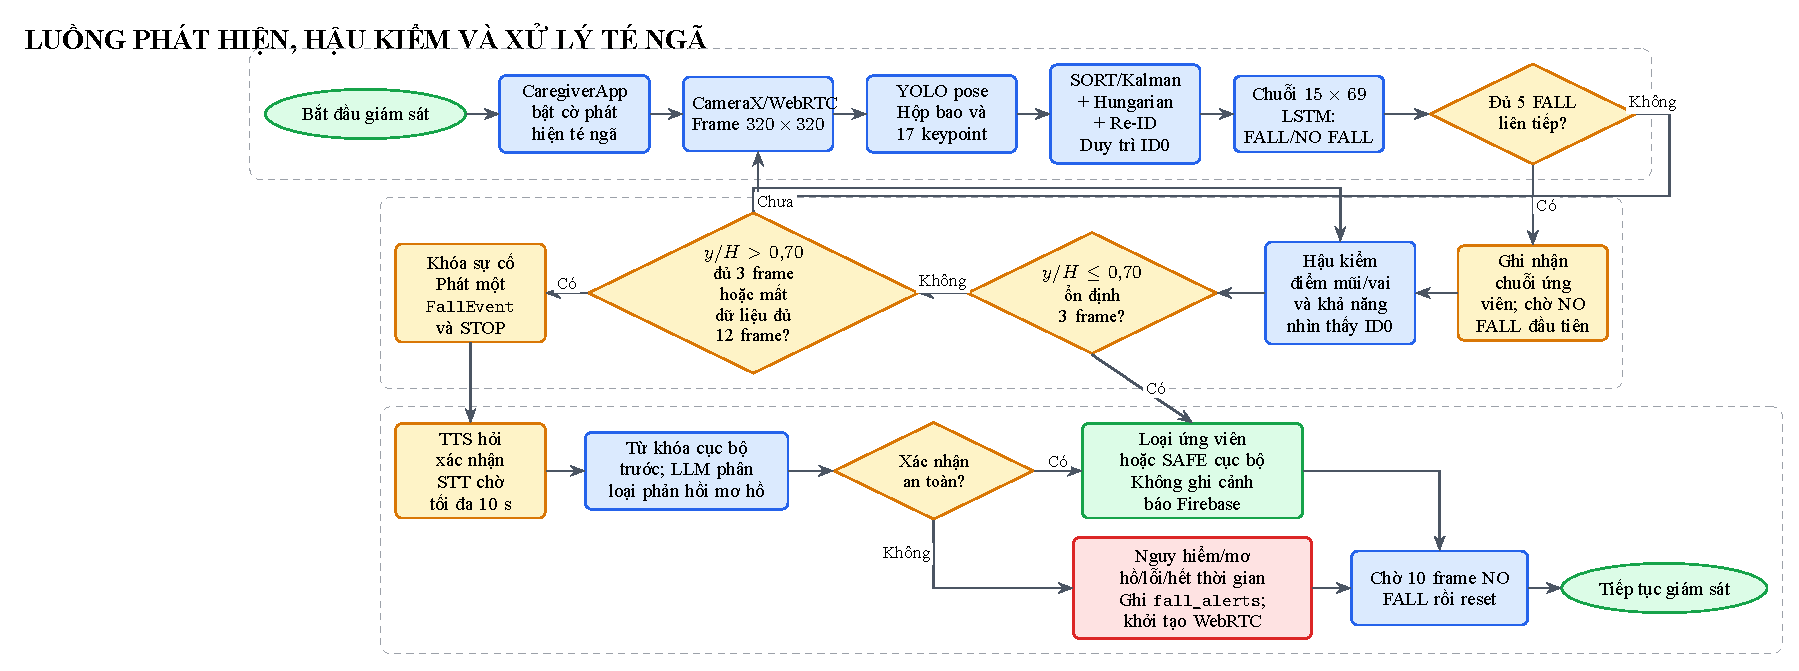
\includegraphics[width=\textwidth]{Images/Activity_Fall_Detection.pdf}
    \caption{Biểu đồ hoạt động của quy trình phát hiện, hậu kiểm và xử lý té ngã}
    \label{fig:activity_fall_detection}
\end{figure}

\clearpage
\subsubsection{Luồng cuộc gọi khẩn cấp và điều khiển từ xa}

Hình \ref{fig:sequence_emergency_response} trình bày quá trình trao đổi giữa người cao tuổi, RobotApp, khối xử lý AI, ESP32, Firebase và CaregiverApp. Khối AI cung cấp kết quả phân tích; RobotApp điều phối việc dừng chuyển động, hỏi xác nhận, lưu cảnh báo và mở màn hình gọi. Khi cần liên lạc, RobotApp ghi \texttt{status=calling}, \texttt{callerRole=robot}, \texttt{emergencyReason=fall} cùng bản mô tả phiên SDP đề nghị vào nhánh báo hiệu của cặp thiết bị. CaregiverApp tiếp nhận yêu cầu gọi và tạo bản mô tả phiên trả lời; hai phía sau đó trao đổi các địa chỉ kết nối ứng viên ICE.

Sau khi kết nối WebRTC được thiết lập, âm thanh và hình ảnh được truyền trực tiếp giữa hai thiết bị hoặc chuyển tiếp qua máy chủ TURN. Khi người chăm sóc sử dụng cần điều khiển ảo, lệnh đi theo chuỗi CaregiverApp $\rightarrow$ RTDB $\rightarrow$ RobotApp $\rightarrow$ BLE $\rightarrow$ ESP32. Các lệnh từ xa vẫn phải qua bước kiểm tra thời điểm tạo lệnh và cơ chế dừng khi không còn cập nhật.

\begin{sidewaysfigure}
    \centering
    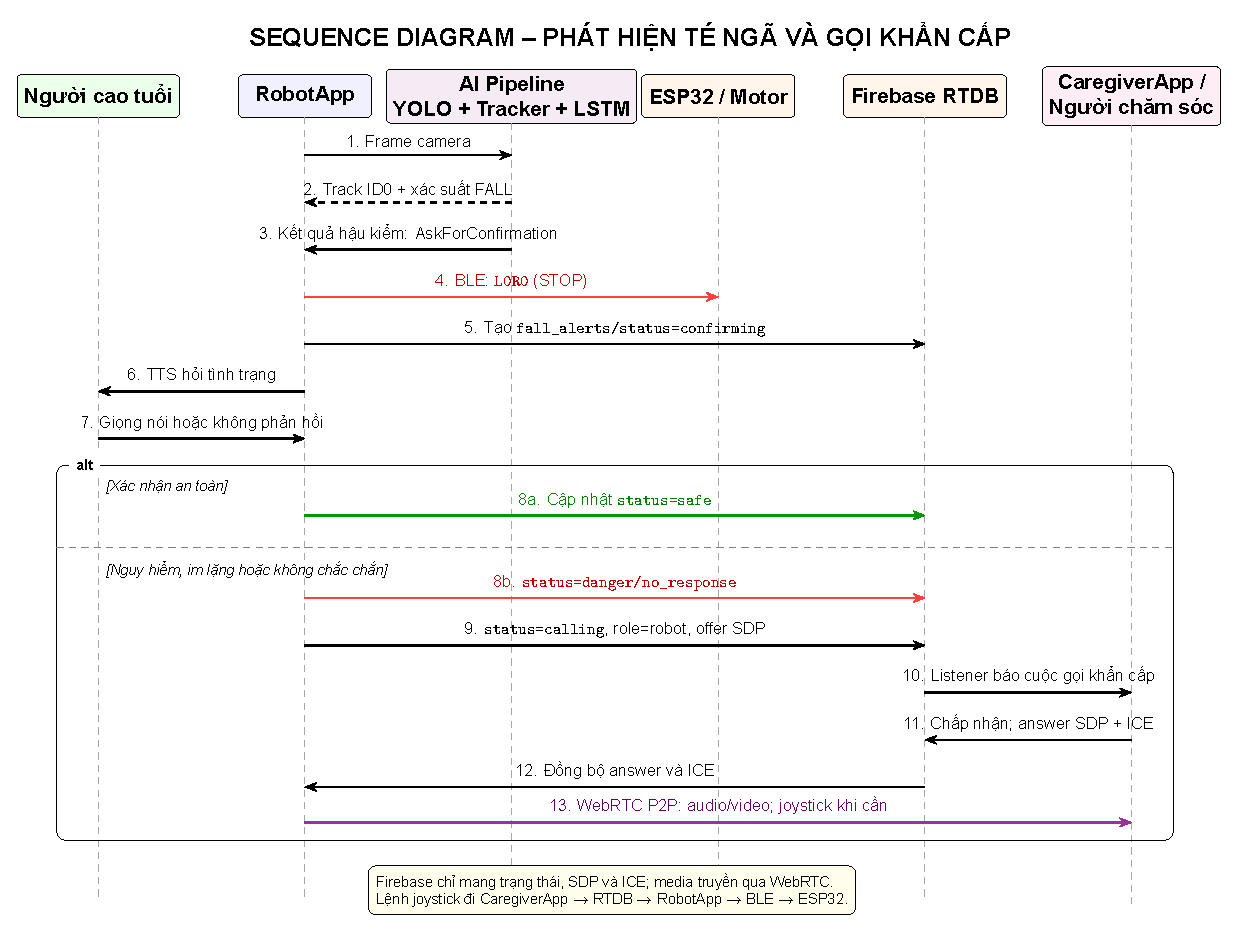
\includegraphics[width=0.92\textheight]{Images/Sequence_Emergency_Response.pdf}
    \caption{Biểu đồ tuần tự của quá trình phát hiện té ngã và thiết lập cuộc gọi khẩn cấp}
    \label{fig:sequence_emergency_response}
\end{sidewaysfigure}

\clearpage
\subsubsection{Luồng hội thoại và nhắc nhở}

Trong hội thoại thông thường, bộ nhận dạng tiếng nói chuyển lời nói thành văn bản. \texttt{GroqChatService} kết hợp câu hỏi với hồ sơ người dùng và lịch sử hội thoại gần nhất để gửi đến LLM, sau đó tiếp nhận từng phần nội dung trả lời. RobotApp ghép các phần này thành câu hoàn chỉnh và đưa vào hàng đợi tổng hợp tiếng nói, nhờ đó có thể bắt đầu trả lời trước khi nhận đủ toàn bộ nội dung. Khi phát xong câu trả lời, ứng dụng trở lại trạng thái lắng nghe.

Đối với lịch nhắc nhở, CaregiverApp lưu cấu hình tại \path|Schedules/{uid}|. \texttt{ReminderService} trên RobotApp kiểm tra lịch mỗi 30 s, đối chiếu thời điểm và chế độ lặp, tạo bản ghi ở trạng thái \texttt{delivered}, rồi gửi sự kiện đến chatbot để phát lời nhắc. LLM hỗ trợ tạo cách diễn đạt thân thiện, trong khi tiêu đề và ghi chú vẫn được lấy từ lịch đã thiết lập. Phản hồi của người dùng và số lần nhắc lại được cập nhật vào cùng bản ghi để người chăm sóc theo dõi.

\subsection{Thiết kế và lựa chọn công nghệ cho các module}

Sau khi xác định các module và luồng phối hợp, những công nghệ phù hợp được lựa chọn dựa trên độ trễ, tài nguyên của điện thoại, khả năng tích hợp và phạm vi hệ thống. Mỗi loại dữ liệu có đặc điểm riêng: giải pháp phù hợp để lưu trữ hồ sơ chưa chắc đáp ứng việc truyền video thời gian thực, còn một mô hình đạt độ chính xác cao trên máy trạm có thể không duy trì được tốc độ suy luận trên điện thoại. Bảng \ref{tab:crosscutting_technology_choices} tóm tắt các quyết định nền tảng; các mục tiếp theo trình bày thiết kế chi tiết của từng khối.

\begin{longtable}{|p{2.8cm}|p{3.4cm}|p{3.5cm}|p{3.8cm}|}
\caption{So sánh các lựa chọn công nghệ xuyên suốt hệ thống}\label{tab:crosscutting_technology_choices}\\
\hline
\textbf{Bài toán} & \textbf{Phương án xem xét} & \textbf{Ưu điểm và hạn chế chính} & \textbf{Lựa chọn cho đề tài} \\
\hline
\endfirsthead
\hline
\textbf{Bài toán} & \textbf{Phương án xem xét} & \textbf{Ưu điểm và hạn chế chính} & \textbf{Lựa chọn cho đề tài} \\
\hline
\endhead
Ứng dụng di động & Phát triển trực tiếp trên Android; nền tảng phát triển đa hệ điều hành; ứng dụng web & Phát triển trực tiếp trên Android thuận tiện khi tích hợp camera, BLE và dịch vụ nền; nền tảng đa hệ điều hành hỗ trợ dùng chung mã giao diện nhưng có thể cần lớp tích hợp riêng & Kotlin, XML và ViewBinding cho hai ứng dụng Android \\
\hline
Suy luận AI & Suy luận trên máy chủ; suy luận tại thiết bị & Máy chủ thuận tiện nâng cấp mô hình nhưng cần truyền ảnh qua mạng; xử lý tại thiết bị giảm phụ thuộc mạng và hạn chế truyền ảnh ra ngoài, song chịu giới hạn tài nguyên & TFLite trên RobotApp, ưu tiên GPU/NNAPI và có CPU dự phòng \reportcite{ref:tflite} \\
\hline
Đồng bộ dữ liệu & REST tự xây dựng; MQTT; cơ sở dữ liệu thời gian thực & REST cho phép kiểm soát cao nhưng cần xây dựng máy chủ; MQTT phù hợp dữ liệu đo và điều khiển nhưng cần broker cùng cơ chế lưu trữ bổ sung; RTDB cung cấp listener và cây JSON nhưng đòi hỏi quản lý chặt cấu trúc dữ liệu và quy tắc truy cập & Firebase Authentication và Realtime Database cho mô hình một cặp thiết bị \reportcite{ref:firebase_rtdb} \\
\hline
Truyền âm thanh và hình ảnh & Truyền qua cơ sở dữ liệu; máy chủ truyền phát tập trung; WebRTC & Cơ sở dữ liệu không phù hợp truyền hình liên tục; máy chủ tập trung cần thêm hạ tầng; WebRTC hỗ trợ liên lạc thời gian thực nhưng cần quản lý báo hiệu và phiên kết nối & WebRTC truyền âm thanh, hình ảnh; RTDB trao đổi thông tin thiết lập cuộc gọi \reportcite{ref:webrtc} \\
\hline
Liên kết điện thoại--thân robot & USB; BLE & USB có độ ổn định cao nhưng ràng buộc thiết bị bằng cáp; BLE phù hợp với các gói lệnh điều khiển có kích thước nhỏ, tiêu thụ ít năng lượng và hỗ trợ kết nối không dây trong phạm vi gần, song có băng thông hạn chế & BLE GATT vì dữ liệu điều khiển có kích thước nhỏ và không bao gồm hình ảnh \reportcite{ref:ble_primer} \\
\hline
Hội thoại & Mô hình cục bộ; LLM qua API; kịch bản cố định & Mô hình cục bộ cần nhiều tài nguyên; LLM qua API hỗ trợ hội thoại linh hoạt nhưng phụ thuộc mạng và chi phí; kịch bản cố định dễ kiểm soát nhưng hạn chế nội dung & Android STT/TTS kết hợp LLM qua API, bổ sung từ khóa nhận biết phản hồi và câu mẫu dự phòng \\
\hline
\end{longtable}

\subsubsection{Module ứng dụng người chăm sóc và điều phối tại robot}

CaregiverApp đảm nhiệm vai trò giao diện quản lý từ xa với bốn nhóm chức năng: hồ sơ và lịch nhắc nhở, cấu hình giám sát, cuộc gọi kèm cần điều khiển ảo, và tra cứu nhật ký. Ứng dụng tiếp nhận thao tác của người chăm sóc, đồng bộ cấu hình, gửi lệnh và xử lý yêu cầu cuộc gọi. Các tác vụ ước lượng tư thế, hội thoại chính và kết nối ESP32 không được đặt tại đây, nhờ đó thiết bị của người chăm sóc không phụ thuộc vào mô hình TFLite hoặc trình điều khiển BLE của robot.

RobotApp điều phối các chức năng trên robot. Ứng dụng tiếp nhận khung hình, âm thanh, lịch nhắc nhở, trạng thái chức năng và lệnh từ xa, sau đó chuyển dữ liệu đến module tương ứng. Kết quả nhận dạng và dự đoán của AI được kết hợp với trạng thái xử lý hiện tại để quyết định dừng robot, hỏi xác nhận hoặc mở cuộc gọi. Kết nối BLE được quản lý tập trung để tránh nhiều thành phần đồng thời tạo kết nối GATT tới ESP32; CameraX và WebRTC luân phiên sử dụng camera theo trạng thái cuộc gọi.

Trong phạm vi đề tài, hai ứng dụng được phát triển trực tiếp trên nền tảng Android bằng Kotlin và XML. Android cung cấp các giao diện lập trình để sử dụng camera, microphone, Bluetooth, nhận dạng và tổng hợp tiếng nói, đồng thời hỗ trợ tổ chức các tác vụ nền. Những khả năng này phù hợp với yêu cầu tích hợp chức năng giám sát, hội thoại và kết nối thân robot. Phần giao diện, xử lý nghiệp vụ và tác vụ nền được phân chia theo chức năng để thuận tiện kiểm thử và bảo trì. Hệ thống hiện hướng đến các thiết bị Android được sử dụng trong đồ án.

\subsubsection{Module thu nhận hình ảnh, ước lượng tư thế và theo dõi mục tiêu}

Để giám sát và phát hiện té ngã trên điện thoại gắn trên robot, module thị giác cần cung cấp đồng thời hộp bao người và các điểm khớp cơ thể với tốc độ phù hợp cho việc phân tích chuyển động theo thời gian. Việc kết hợp một bộ phát hiện người với một mô hình ước lượng tư thế riêng cho phép thay thế từng thành phần độc lập, nhưng cần hai lượt suy luận và bước chuyển vùng ảnh giữa hai mô hình. Mô hình tích hợp phát hiện người và ước lượng tư thế tạo cả hai loại kết quả trong cùng một lượt suy luận, giúp đơn giản hóa chuỗi xử lý.

Các mô hình MobileNet SSD và EfficientDet tiêu chuẩn phục vụ phát hiện đối tượng nhưng không trực tiếp cung cấp 17 điểm khớp, nên cần thêm mô hình ước lượng tư thế. YOLO-Pose cung cấp đồng thời hộp bao và điểm khớp, đồng thời hỗ trợ xuất sang TFLite/LiteRT \reportcite{ref:yolo_pose_docs}. Từ quy trình ở Mục \ref{sec:yolo_pose_inference_pipeline}, cấu trúc đầu vào, đầu ra ở Mục \ref{sec:yolo_pose_output_representation} và so sánh quy mô ở Mục \ref{sec:yolo26_pose_scales}, đề tài lựa chọn YOLO26n-Pose. Biến thể nano có số tham số và chi phí tính toán thấp nhất trong các mức n, s, m, l và x, phù hợp với điện thoại còn phải thực hiện theo dõi, hội thoại, đồng bộ dữ liệu và điều khiển. Tuy nhiên, chỉ số mAP ước lượng tư thế thấp hơn các biến thể lớn, nên lựa chọn này cần được đánh giá thêm về độ trễ và chất lượng điểm khớp trên thiết bị sử dụng.

Module nhận khung hình từ CameraX hoặc bản sao hình ảnh của WebRTC. Ảnh được đổi về kích thước $320\times320$ trước khi suy luận bằng YOLO-Pose. Kết quả được lọc với ngưỡng tin cậy 0,20, ngưỡng IoU của bước NMS là 0,45 và ngưỡng hiển thị điểm khớp là 0,30. Hộp bao người và 17 điểm khớp được dùng chung cho theo dõi mục tiêu, ước lượng độ gần và phân tích bằng LSTM. Tần suất xử lý được đặt giới hạn trên ở 25 FPS; nếu lượt suy luận trước chưa hoàn tất, khung hình mới được bỏ qua để hạn chế tích lũy độ trễ.

Việc gửi khung hình lên dịch vụ đám mây cho phép sử dụng phần cứng mạnh hơn, nhưng làm tăng độ trễ, băng thông và rủi ro đối với dữ liệu hình ảnh. Suy luận trực tiếp trên điện thoại chịu giới hạn về tài nguyên nhưng đáp ứng tốt hơn NFR02, NFR06 và vẫn hoạt động khi Internet gián đoạn. Vì vậy, TFLite được chọn làm môi trường suy luận trên thiết bị; hệ thống ưu tiên GPU, chuyển sang NNAPI khi cần và sử dụng CPU bốn luồng làm phương án cuối \reportcite{ref:tflite}.

Đối với theo dõi người, SORT có cấu trúc gọn và tốc độ xử lý cao nhưng phụ thuộc vào chất lượng phát hiện. ByteTrack tận dụng thêm các kết quả có độ tin cậy thấp để duy trì đối tượng khi bị che khuất, đồng thời cần thêm bước liên kết kết quả \reportcite{ref:sort}\reportcite{ref:bytetrack}. Mạng tái định danh dựa trên học sâu có thể phân biệt ngoại hình tốt hơn, nhưng làm tăng dung lượng mô hình và thời gian suy luận. Đề tài sử dụng cấu trúc SORT với bộ lọc Kalman và thuật toán Hungarian, bổ sung khoảng cách giữa các điểm khớp và biểu đồ phân bố màu H--S khi cần nhận lại mục tiêu. Hàm chi phí liên kết được xác định như sau:

\begin{equation}
C=0,30(1-\operatorname{IoU})+0,30\hat d_c+0,30\hat d_p+0,10p_a,
\end{equation}

trong đó $\hat d_c$ là khoảng cách tâm đã chuẩn hóa, $\hat d_p$ là khoảng cách giữa các điểm mốc tại vai và hông, còn $p_a$ là thành phần chi phí phản ánh sự thay đổi diện tích hộp bao. Khi lựa chọn người mục tiêu ban đầu, mỗi đối tượng được đánh giá theo điểm số:

\begin{equation}
Q=0,60q_{area}+0,15q_{det}+0,15q_{vis}+0,10q_{center}-p_{edge}.
\end{equation}

Trong biểu thức trên, $q_{area}$ phản ánh diện tích hộp bao, $q_{det}$ là độ tin cậy phát hiện, $q_{vis}$ phản ánh tỷ lệ điểm khớp quan sát được, $q_{center}$ biểu diễn mức độ gần tâm ảnh và $p_{edge}$ là thành phần giảm điểm khi người bị cắt ở biên ảnh. Đối tượng có điểm số cao nhất được gán định danh ID0 để dùng chung cho bám theo và phát hiện té ngã. Bộ theo dõi duy trì ID0 tối đa 45 khung hình không ghép được với kết quả phát hiện; các định danh khác được giữ tối đa 10 khung hình. Cơ chế tìm lại mục tiêu hoạt động trong khoảng 2 s, với điều kiện đối tượng nằm cách vị trí cuối không quá 35\% đường chéo ảnh, thuộc vùng trung tâm và được quan sát ổn định trong ba khung hình. Khi đang xử lý một sự kiện nghi té ngã, hệ thống không tự chuyển sang người khác.

\subsubsection{Module tự bám theo và điều khiển chuyển động}

Module bám theo tự động nhận hộp bao và các điểm khớp của mục tiêu ID0, sau đó tạo vector điều khiển tịnh tiến và quay đã chuẩn hóa. Độ gần được ước lượng từ diện tích hộp bao và các mốc vai, hông, gối, mắt cá chân, rồi làm mượt bằng trung bình trượt lũy thừa (Exponential Moving Average -- EMA). Giá trị này được chia thành ba vùng: quá xa, phù hợp và quá gần. Ngưỡng đi vào và rời khỏi mỗi vùng được đặt khác nhau để hạn chế việc robot đổi trạng thái liên tục khi giá trị dao động gần biên. Sai lệch ngang giữa tâm mục tiêu và tâm ảnh tạo thành phần quay, với vùng chết 0,07, hệ số 2,2 và giới hạn độ lớn 0,50. Vector điều khiển được cập nhật khoảng mỗi 120 ms.

Bộ điều khiển chỉ dựa vào tâm hộp bao có chi phí tính toán thấp, nhưng có thể đánh giá sai khoảng cách khi phần chân bị cắt khỏi ảnh. Cảm biến chiều sâu cung cấp khoảng cách trực tiếp hơn nhưng làm tăng độ phức tạp phần cứng và nằm ngoài phạm vi đề tài. Do đó, hệ thống kết hợp hộp bao với các keypoint và áp dụng chính sách chuyển động thận trọng: khi vùng bao quá lớn hoặc phần chân không còn trong khung hình, robot ưu tiên lùi để quan sát đầy đủ hơn. Sau khi xuất hiện kết quả FALL, robot không tiến về phía người mà chỉ dừng, lùi chậm hoặc quay tại chỗ; nếu mất ID0 trong trạng thái này, robot dừng ngay.

Lệnh từ cần điều khiển ảo và chức năng bám theo tự động sử dụng chung cấu trúc $x,y,ts$, nhưng chỉ một nguồn được quyền điều khiển tại một thời điểm. Module cầu nối tập trung việc kiểm tra thời điểm tạo lệnh, giới hạn giá trị và dừng khi quá thời gian chờ, giúp áp dụng cùng một quy trình kiểm tra cho cả hai nguồn.

\subsubsection{Module phát hiện, hậu kiểm và xác nhận té ngã}

Bài toán phát hiện té ngã có thể được tiếp cận bằng ngưỡng hình học trên từng khung hình, mô hình phân loại trực tiếp từ ảnh hoặc đoạn video, hoặc mô hình phân tích chuỗi điểm khớp. Ngưỡng hình học có chi phí tính toán thấp và dễ giải thích nhưng nhạy với góc nhìn. Mô hình học trực tiếp từ video có thể khai thác cả hình ảnh và chuyển động, song cần nhiều tài nguyên và dữ liệu huấn luyện. Chuỗi điểm khớp có kích thước đầu vào nhỏ hơn và thể hiện được diễn biến tư thế, nhưng phụ thuộc vào chất lượng ước lượng các điểm này. Đề tài lựa chọn YOLO-Pose kết hợp LSTM, sau đó kiểm tra bổ sung theo quy tắc và hỏi xác nhận bằng giọng nói để hạn chế cảnh báo nhầm.

Mỗi khung hình của mục tiêu ID0 được chuyển thành vector 69 đặc trưng:

\begin{equation}
\mathbf f_t=[x_i,y_i,\Delta x_i,\Delta y_i]_{i=1}^{17}\oplus r_t,
\end{equation}

trong đó tọa độ điểm khớp được chuẩn hóa theo tâm hông và kích thước vùng tư thế, $\Delta x_i,\Delta y_i$ là độ dịch chuyển so với khung hình trước, còn $r_t$ là tỷ lệ rộng/cao. Cửa sổ 15 khung hình tạo tensor $[1,15,69]$; LSTM trả về $[p_{normal},p_{fall}]$ và kết quả được gán nhãn FALL khi $p_{fall}>p_{normal}$. LSTM khai thác quan hệ theo thời gian của chuỗi tư thế để bổ sung thông tin chuyển động cho việc phân loại \reportcite{ref:lstm}.

Bộ hậu kiểm quản lý quá trình xử lý qua các trạng thái \texttt{MONITORING}, \texttt{FALL\_SEQUENCE}, \texttt{VERIFYING}, \texttt{PROMPTED}, \texttt{DISMISSED} và \texttt{CONFIRMED}, tương ứng với giám sát, ghi nhận chuỗi nghi té ngã, kiểm tra bổ sung, hỏi xác nhận, loại bỏ sự kiện và xác nhận nguy hiểm. Năm kết quả FALL liên tiếp hình thành một chuỗi nghi té ngã. Sau kết quả NO FALL đầu tiên, ba khung hình liên tiếp có điểm mũi hoặc vai ở $y/H\leq0,70$ sẽ loại bỏ sự kiện; ba khung hình liên tiếp có các điểm này ở $y/H>0,70$, hoặc 12 khung hình liên tiếp không quan sát được mục tiêu hay phần thân trên, sẽ dẫn đến bước hỏi xác nhận. Nếu câu trả lời chưa rõ nghĩa, xảy ra lỗi phân loại hoặc hết 10 s chờ phản hồi, hệ thống xử lý theo trường hợp cần hỗ trợ. Sau khi sự kiện được kết luận, bộ hậu kiểm chỉ trở về trạng thái giám sát khi ghi nhận 10 kết quả NO FALL liên tiếp, nhằm hạn chế yêu cầu xác nhận trùng lặp. Các bước kiểm tra bổ sung tạo thêm độ trễ, đổi lại giúp hệ thống xem xét diễn biến qua nhiều khung hình trước khi phát cảnh báo.

\subsubsection{Module hội thoại và lời nhắc}

Mô hình hội thoại chạy hoàn toàn tại thiết bị hạn chế phụ thuộc mạng và việc gửi dữ liệu ra ngoài, nhưng cần chia sẻ tài nguyên với chức năng thị giác. Phương án dùng kịch bản cố định có chi phí xử lý thấp và dễ kiểm soát nội dung, song khó đáp ứng hội thoại hằng ngày với nhiều chủ đề. Vì vậy, đề tài kết hợp Android SpeechRecognizer để chuyển tiếng nói thành văn bản, LLM qua API để tạo câu trả lời và Android TextToSpeech để tổng hợp tiếng nói \reportcite{ref:android_speech}\reportcite{ref:groq_api}\reportcite{ref:android_tts}. Những phản hồi thể hiện rõ tình trạng an toàn hoặc nguy hiểm được nhận biết trước bằng từ khóa tại thiết bị; chức năng nhắc nhở sử dụng câu mẫu dự phòng khi không nhận được phản hồi từ API.

Hoạt động hội thoại được tổ chức theo các trạng thái nghỉ, lắng nghe, xử lý câu hỏi, phát câu trả lời, xác nhận lời nhắc, xác nhận té ngã và đang gọi. Hồ sơ người dùng được bổ sung vào phần chỉ dẫn cho LLM; lịch sử hội thoại giới hạn ở 20 thông điệp để kiểm soát độ dài ngữ cảnh. Phản hồi được tiếp nhận từng phần, ghép thành câu rồi đưa vào TTS, giúp rút ngắn thời gian từ khi đặt câu hỏi đến khi robot bắt đầu trả lời. Các tác vụ ngắn, như phân loại phản hồi hoặc nhận biết yêu cầu gọi, sử dụng yêu cầu riêng nhận kết quả đầy đủ trong một lần và không thêm vào lịch sử trò chuyện. Module nhắc nhở kiểm tra lịch mỗi 30 s, tạo bản ghi trước khi phát sự kiện và giữ nguyên nội dung lịch đã thiết lập.

\subsubsection{Module dữ liệu dùng chung và liên lạc thời gian thực}

Firebase Realtime Database được lựa chọn để đồng bộ các dữ liệu có kích thước nhỏ như trạng thái chức năng, lệnh điều khiển và sự kiện. Các bộ lắng nghe thông báo thay đổi đến hai ứng dụng gần thời gian thực, kết hợp với Firebase Authentication để xác định tài khoản truy cập. Giải pháp này giảm khối lượng xây dựng máy chủ riêng so với REST hoặc việc bổ sung cơ chế lưu trữ cho MQTT. Tuy nhiên, hai ứng dụng cần thống nhất cấu trúc cây JSON và đường dẫn; việc thay đổi cấu trúc dữ liệu phải được cập nhật đồng bộ. Các đường dẫn vì vậy được quản lý tập trung và phân vùng theo UID; lệnh điều khiển kèm thời điểm tạo để kiểm tra hiệu lực. Hai thiết bị dùng chung tài khoản nên hệ thống hiện chưa phân quyền riêng cho robot và người chăm sóc \reportcite{ref:firebase_rtdb}\reportcite{ref:firebase_security}.

Âm thanh và hình ảnh được truyền bằng WebRTC, còn RTDB lưu trạng thái và thông tin thiết lập cuộc gọi, gồm bản mô tả phiên đề nghị, bản trả lời và hai nhánh địa chỉ ứng viên ICE. WebRTC hỗ trợ kết nối trực tiếp khi điều kiện mạng cho phép và chuyển tiếp qua TURN khi cần. Quá trình tích hợp phải quản lý đồng thời kết nối, báo hiệu, thời gian chờ và quyền sử dụng camera \reportcite{ref:webrtc}\reportcite{ref:ice}. Yêu cầu gọi được hủy nếu không được chấp nhận sau 30 s. Ngoài cuộc gọi, CameraX cung cấp hình ảnh xem trước và khung hình phân tích. Trong cuộc gọi, CameraX được ngắt liên kết; WebRTC sử dụng camera và gửi bản sao khung hình cục bộ đến khối AI.

\subsubsection{Module cầu nối BLE và chấp hành thân robot}

Dữ liệu gửi đến thân robot chỉ gồm vận tốc đặt của hai bánh, có kích thước nhỏ và không chứa hình ảnh. BLE GATT đáp ứng nhu cầu trao đổi này trong phạm vi gần, đồng thời cho phép kết nối không dây giữa điện thoại và ESP32. Khi sử dụng thao tác ghi không phản hồi, phía gửi không nhận xác nhận ở mức GATT cho từng lệnh. Vì vậy, hệ thống kết hợp kiểm tra thời hạn lệnh và cơ chế tự dừng khi không nhận cập nhật, bên cạnh việc chủ động gửi lệnh dừng \reportcite{ref:ble_primer}.

Module cầu nối kiểm tra thời điểm tạo lệnh, giới hạn giá trị và chuyển vector điều khiển thành chuỗi \texttt{L...R...} để gửi qua BLE. ESP32 đóng vai trò máy chủ GATT, xử lý vùng không đáp ứng, giới hạn vận tốc đặt và điều khiển hai động cơ BLDC. Hai cảm biến góc AS5600 kết nối qua hai bus I2C riêng; mỗi mạch công suất nhận ba tín hiệu PWM. Các thông số thiết kế gồm 7 cặp cực cho mỗi động cơ, điện áp nguồn 17,5 V, giới hạn điện áp điều khiển 10 V và vận tốc 40 rad/s. Bộ điều khiển vận tốc sử dụng $P=0,1$, $I=1,0$, $D=0$ và bộ lọc có hằng số thời gian $T_f=0,01$ s. Thư viện SimpleFOC cung cấp các hàm khởi tạo và cập nhật điều khiển FOC vòng kín, giúp thuận tiện tích hợp phần cứng; các tham số vẫn cần được hiệu chỉnh theo đặc điểm cơ khí của robot \reportcite{ref:foc}\reportcite{ref:simplefoc}.

\subsubsection{Module chuẩn bị và triển khai mô hình AI}

Trước khi tích hợp vào Android, mô hình YOLO-Pose được chuyển từ PyTorch sang ONNX với đầu vào cố định $320\times320$, sau đó qua \texttt{onnx2tf}/SavedModel để tạo tệp TFLite. Mô hình LSTM được chuyển từ Keras H5 sang TFLite với tập toán tử \texttt{SELECT\_TF\_OPS}. Biến thể YOLO có đầu ra thô, không tích hợp NMS, được ưu tiên cho suy luận bằng GPU; biến thể đầu cuối (E2E) có bước lựa chọn dự đoán được dùng làm phương án dự phòng. Khi nạp mô hình, ứng dụng đọc kích thước tensor để xử lý hai dạng đầu ra \texttt{[1,56,2100]} và \texttt{[1,300,57]}.

ONNX đóng vai trò định dạng trung gian giữa môi trường huấn luyện và TensorFlow; TFLite là định dạng triển khai trên Android và hỗ trợ sử dụng các bộ tăng tốc phần cứng. Quá trình chuyển đổi có thể làm thay đổi toán tử hoặc quy ước đầu ra, nên thiết kế bao gồm bước kiểm tra kích thước tensor và so sánh kết quả suy luận trước khi đóng gói. Việc lưu cấu hình dữ liệu, tham số huấn luyện, phiên bản mô hình và mã băm của tệp cũng cần được thực hiện thống nhất để có thể lặp lại quy trình khi thay đổi mô hình.

\subsection{Thiết kế dữ liệu, giao thức truyền thông và phương thức kết nối}

\subsubsection{Cây dữ liệu Firebase}

Firebase RTDB lưu dữ liệu theo cấu trúc cây JSON và chuyển thay đổi đến các bộ lắng nghe của hai ứng dụng \reportcite{ref:firebase_rtdb}. Dữ liệu vận hành của từng cặp thiết bị được gom dưới \path|pair_sessions/{uid}|, trong khi hồ sơ, lịch và nhật ký lời nhắc được tổ chức thành các nhánh theo UID ở cấp gốc.

\begin{longtable}{|p{4.5cm}|p{4.2cm}|p{4.8cm}|}
\caption{Cấu trúc dữ liệu của Firebase Realtime Database}\label{tab:rtdb_schema}\\
\hline
\textbf{Đường dẫn} & \textbf{Trường chính} & \textbf{Mục đích} \\
\hline
\endfirsthead
\hline
\textbf{Đường dẫn} & \textbf{Trường chính} & \textbf{Mục đích} \\
\hline
\endhead
\path|Users/{uid}| & fullName, robotName, pronoun, caregiver, medicalConditions, notes, hobbies & Hồ sơ và ngữ cảnh hội thoại \\
\hline
\path|Schedules/{uid}/{id}| & title, note, dateMillis, hour, minute, repeatMode, active & Lịch một lần hoặc lặp \\
\hline
\path|reminder_logs/{uid}/{id}| & scheduleId, triggeredAt, status, elderlyResponse, retryCount, confirmedAt & Nhật ký thực thi lời nhắc \\
\hline
\path|pair_sessions/{uid}/robot_follow_enabled| & Boolean & Bật/tắt auto-follow \\
\hline
\path|pair_sessions/{uid}/ai_fall_detection_enabled| & Boolean & Bật/tắt LSTM/hậu kiểm \\
\hline
\path|pair_sessions/{uid}/robot_control| & x, y, ts & Lệnh joystick hoặc auto-follow \\
\hline
\path|pair_sessions/{uid}/webrtc_signal| & status, callerRole, emergencyReason, offer, answer, robotCandidates, caregiverCandidates & Signaling và trạng thái cuộc gọi \\
\hline
\path|pair_sessions/{uid}/fall_alerts/{pushId}| & timestamp, trackId, probFall, verificationReason, confirmationStatus, severity, evidence & Cảnh báo nguy hiểm/không phản hồi \\
\hline
\path|pair_sessions/{uid}/call_history/{pushId}| & timestamp, initiator, durationSec, status & Nhật ký cuộc gọi \\
\hline
\end{longtable}

Quy tắc bảo mật mặc định đặt \texttt{.read=false} và \texttt{.write=false}; mỗi nhánh chỉ cho phép truy cập khi \texttt{auth != null} và \texttt{auth.uid === \$uid}. Hai nhánh lịch sử được lập chỉ mục theo thời điểm để hỗ trợ truy vấn. Các quy tắc này giới hạn người dùng vào vùng dữ liệu thuộc UID tương ứng \reportcite{ref:firebase_security}. Tuy nhiên, robot và người chăm sóc chưa có quyền truy cập riêng vì hai thiết bị đang sử dụng cùng tài khoản.

\subsubsection{Cấu trúc dữ liệu điều khiển trên RTDB}

\begin{lstlisting}[caption={Cấu trúc lệnh điều khiển trong phiên ghép cặp}]
pair_sessions/{uid}/robot_control = {
  "x": Number,   // translation, [-1, 1]
  "y": Number,   // steering,    [-1, 1]
  "ts": Long     // Unix epoch milliseconds
}
\end{lstlisting}

Trong CaregiverApp, độ lệch joystick được chuẩn hóa theo bán kính $r$:

\begin{equation}
x=\frac{\Delta y}{r}, \qquad y=-\frac{\Delta x}{r}.
\end{equation}

Do tọa độ $y$ trên màn hình tăng theo chiều từ trên xuống, thao tác kéo lên tạo $x<0$. RobotApp tiếp nhận lệnh khi $x,y$ là các giá trị hữu hạn, có thời điểm tạo lệnh, tuổi lệnh không quá 2.000 ms và thời điểm này không vượt quá thời gian hiện tại hơn 5.000 ms. Sau khi giới hạn $x,y$ trong $[-1,1]$, vận tốc đặt của hai động cơ được tính như sau:

\begin{align}
t &= \operatorname{clip}(x,-1,1),\\
s &= 0,15\operatorname{clip}(y,-1,1),\\
v_L &= (s+t)20,\\
v_R &= (s-t)20.
\end{align}

Nếu $|x|>0,3$ và $|y|<0,3$, thành phần quay được đưa về 0 để giảm dao động khi đi thẳng. Do hai động cơ được lắp đối xứng, dấu của vận tốc đặt tuân theo chiều trục động cơ đã hiệu chỉnh. Vì vậy, hướng chuyển động của robot phải được xác định theo quy ước lắp đặt, không chỉ dựa vào việc hai giá trị vận tốc cùng dấu hay trái dấu.

\begin{table}[htbp]
\centering
\caption{Các điểm chuẩn ánh xạ lệnh điều khiển}
\label{tab:motor_mapping}
\begin{tabular}{|c|c|c|c|}
\hline
$x$ & $y$ & $(v_L,v_R)$ & Ý nghĩa hiệu chỉnh \\
\hline
$-1$ & $0$ & $(-20,20)$ & Tiến \\
\hline
$1$ & $0$ & $(20,-20)$ & Lùi \\
\hline
$0$ & $1$ & $(3,3)$ & Quay theo chiều dương \\
\hline
$0$ & $-1$ & $(-3,-3)$ & Quay theo chiều âm \\
\hline
$0$ & $0$ & $(0,0)$ & Dừng \\
\hline
\end{tabular}
\end{table}

\subsubsection{Giao tiếp BLE và điều khiển động cơ trên ESP32}

RobotApp đóng vai trò máy khách GATT, còn ESP32 là máy chủ GATT có tên \texttt{OhmniRobot}. Mã định danh dịch vụ là \texttt{4FAFC201-\allowbreak 1FB5-\allowbreak 459E-\allowbreak 8FCC-\allowbreak C5C9C331914B}; đặc tính nhận lệnh có UUID \texttt{BEB5483E-\allowbreak 36E1-\allowbreak 4688-\allowbreak B7F5-\allowbreak EA07361B26A8}. Gói lệnh là chuỗi ASCII dạng \texttt{L<float>R<float>\textbackslash n}, định dạng số theo \texttt{Locale.US} và được gửi bằng thao tác ghi không phản hồi \path|WRITE_NO_RESPONSE|. Cách tổ chức dịch vụ và đặc tính tuân theo mô hình GATT \reportcite{ref:ble_primer}.

Firmware đưa giá trị có độ lớn dưới 0,5 về 0, nâng độ lớn của giá trị khác 0 nhưng nhỏ hơn 3 lên 3, rồi giới hạn kết quả trong $[-40,40]$. Trong mỗi vòng lặp, chương trình gọi \texttt{loopFOC()} cho hai động cơ, kiểm tra thời gian nhận lệnh và truyền vận tốc đặt vào \texttt{move()}. Khi kết nối BLE bị ngắt, hàm xử lý sự kiện đặt vận tốc của cả hai động cơ về 0. Bộ phân tích lệnh hiện xác định vị trí ký tự L/R rồi chuyển chuỗi thành số bằng \texttt{toFloat}; việc kiểm tra toàn bộ chuỗi và loại giá trị không hợp lệ tại ESP32 vẫn cần được bổ sung để hoàn thiện cơ chế tiếp nhận lệnh.

\subsubsection{Cơ chế dừng an toàn nhiều tầng}

Hệ thống kết hợp bốn cơ chế dừng theo vị trí xử lý trong chuỗi điều khiển:

\begin{enumerate}
    \item Ứng dụng gửi lệnh dừng khi người dùng thả cần điều khiển, ẩn phần điều khiển, tắt bám theo tự động hoặc kết thúc cuộc gọi.
    \item RobotApp loại bản cập nhật RTDB quá 2 s, sai kiểu hoặc chứa giá trị không hữu hạn.
    \item Bộ giám sát thời gian nhận lệnh trong \texttt{RobotControlManager} gửi \texttt{L0R0} sau 500 ms không nhận cập nhật.
    \item Firmware đưa vận tốc đặt của hai động cơ về 0 sau 800 ms không nhận lệnh hoặc ngay khi kết nối BLE bị ngắt.
\end{enumerate}

Cơ chế giám sát thời gian nhận lệnh, thường gọi là watchdog, được đặt ở cả ứng dụng và ESP32. Ngưỡng trên Android ngắn hơn ngưỡng ở firmware để ứng dụng chủ động gửi lệnh dừng trước. ESP32 tiếp tục kiểm tra độc lập và đưa vận tốc về 0 nếu ứng dụng bị treo hoặc kết nối bị ngắt trước khi lệnh dừng được truyền đến.

\subsection{Kết luận chương}

Chương đã xác định phạm vi, yêu cầu chức năng và yêu cầu chất lượng làm cơ sở phân chia nhiệm vụ cho RobotApp, CaregiverApp, dịch vụ dùng chung và phần thân robot. Trên kiến trúc tổng quan đó, các luồng giám sát, hội thoại, nhắc nhở, liên lạc và điều khiển được phân tích để lựa chọn công nghệ phù hợp. Thiết kế cũng xác định cách chuẩn bị mô hình AI, tổ chức dữ liệu, truyền nhận lệnh và phối hợp các cơ chế dừng an toàn. Những nội dung này là cơ sở để hiện thực hệ thống ở Chương 4 và đánh giá kết quả ở Chương 5.
